% !TEX TS-program = pdflatex
% !TEX encoding = UTF-8 Unicode
\documentclass[border=0mm]{standalone}
% packages
\usepackage{tikz}
\usetikzlibrary{patterns}
\usepackage{amsmath,amssymb}
\usepackage{bm}
\usepackage{pgfplots}
\pgfplotsset{compat=1.15}
% start document
\begin{document}
% generated by ROOT (CERN)
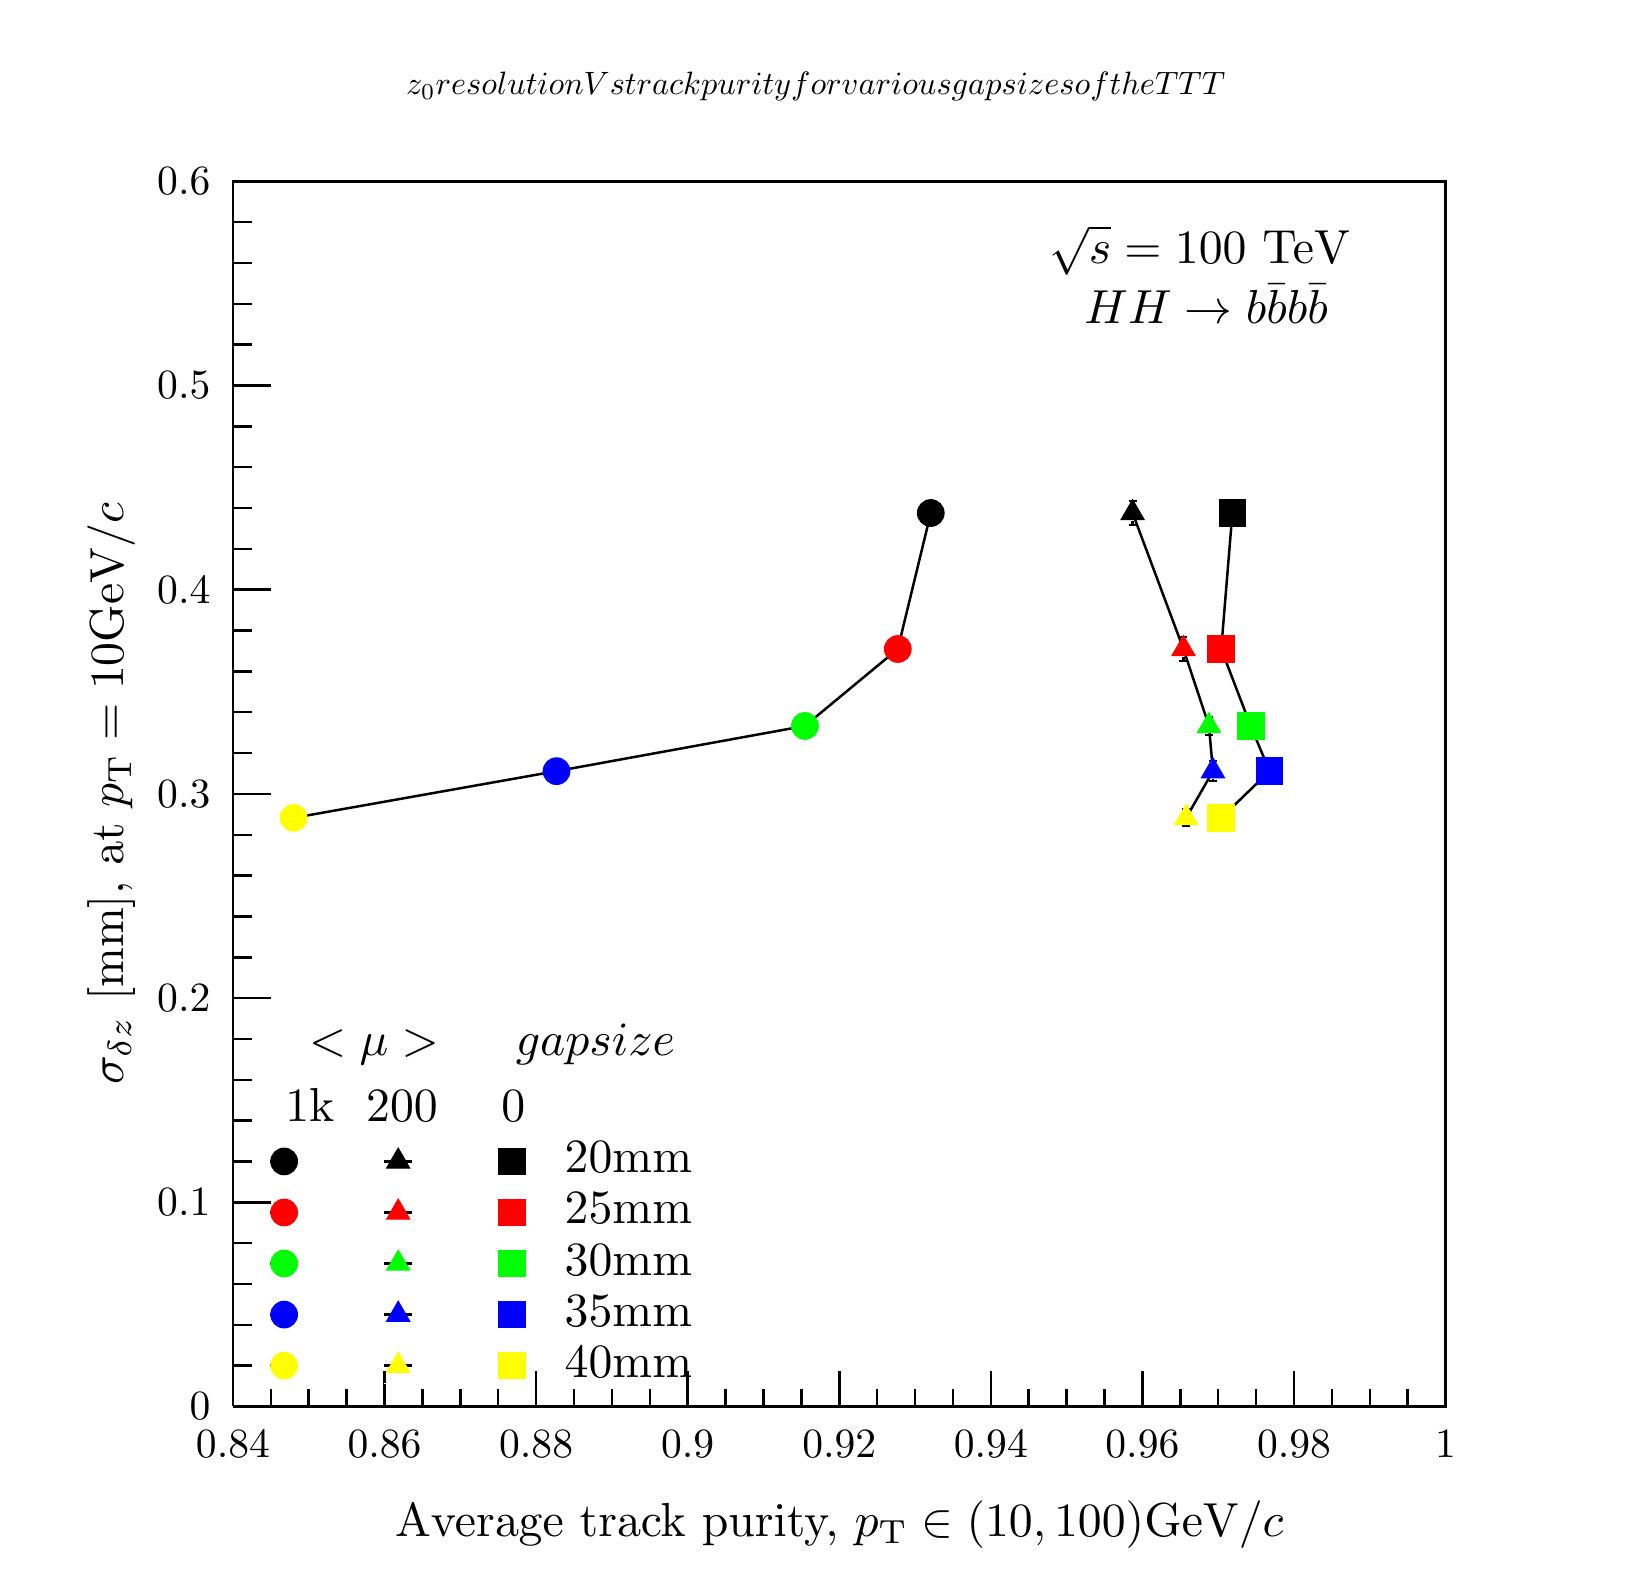
\begin{tikzpicture}
\pgfdeclareplotmark{cross} {
\pgfpathmoveto{\pgfpoint{-0.3\pgfplotmarksize}{\pgfplotmarksize}}
\pgfpathlineto{\pgfpoint{+0.3\pgfplotmarksize}{\pgfplotmarksize}}
\pgfpathlineto{\pgfpoint{+0.3\pgfplotmarksize}{0.3\pgfplotmarksize}}
\pgfpathlineto{\pgfpoint{+1\pgfplotmarksize}{0.3\pgfplotmarksize}}
\pgfpathlineto{\pgfpoint{+1\pgfplotmarksize}{-0.3\pgfplotmarksize}}
\pgfpathlineto{\pgfpoint{+0.3\pgfplotmarksize}{-0.3\pgfplotmarksize}}
\pgfpathlineto{\pgfpoint{+0.3\pgfplotmarksize}{-1.\pgfplotmarksize}}
\pgfpathlineto{\pgfpoint{-0.3\pgfplotmarksize}{-1.\pgfplotmarksize}}
\pgfpathlineto{\pgfpoint{-0.3\pgfplotmarksize}{-0.3\pgfplotmarksize}}
\pgfpathlineto{\pgfpoint{-1.\pgfplotmarksize}{-0.3\pgfplotmarksize}}
\pgfpathlineto{\pgfpoint{-1.\pgfplotmarksize}{0.3\pgfplotmarksize}}
\pgfpathlineto{\pgfpoint{-0.3\pgfplotmarksize}{0.3\pgfplotmarksize}}
\pgfpathclose
\pgfusepathqstroke
}
\pgfdeclareplotmark{cross*} {
\pgfpathmoveto{\pgfpoint{-0.3\pgfplotmarksize}{\pgfplotmarksize}}
\pgfpathlineto{\pgfpoint{+0.3\pgfplotmarksize}{\pgfplotmarksize}}
\pgfpathlineto{\pgfpoint{+0.3\pgfplotmarksize}{0.3\pgfplotmarksize}}
\pgfpathlineto{\pgfpoint{+1\pgfplotmarksize}{0.3\pgfplotmarksize}}
\pgfpathlineto{\pgfpoint{+1\pgfplotmarksize}{-0.3\pgfplotmarksize}}
\pgfpathlineto{\pgfpoint{+0.3\pgfplotmarksize}{-0.3\pgfplotmarksize}}
\pgfpathlineto{\pgfpoint{+0.3\pgfplotmarksize}{-1.\pgfplotmarksize}}
\pgfpathlineto{\pgfpoint{-0.3\pgfplotmarksize}{-1.\pgfplotmarksize}}
\pgfpathlineto{\pgfpoint{-0.3\pgfplotmarksize}{-0.3\pgfplotmarksize}}
\pgfpathlineto{\pgfpoint{-1.\pgfplotmarksize}{-0.3\pgfplotmarksize}}
\pgfpathlineto{\pgfpoint{-1.\pgfplotmarksize}{0.3\pgfplotmarksize}}
\pgfpathlineto{\pgfpoint{-0.3\pgfplotmarksize}{0.3\pgfplotmarksize}}
\pgfpathclose
\pgfusepathqfillstroke
}
\pgfdeclareplotmark{newstar} {
\pgfpathmoveto{\pgfqpoint{0pt}{\pgfplotmarksize}}
\pgfpathlineto{\pgfqpointpolar{44}{0.5\pgfplotmarksize}}
\pgfpathlineto{\pgfqpointpolar{18}{\pgfplotmarksize}}
\pgfpathlineto{\pgfqpointpolar{-20}{0.5\pgfplotmarksize}}
\pgfpathlineto{\pgfqpointpolar{-54}{\pgfplotmarksize}}
\pgfpathlineto{\pgfqpointpolar{-90}{0.5\pgfplotmarksize}}
\pgfpathlineto{\pgfqpointpolar{234}{\pgfplotmarksize}}
\pgfpathlineto{\pgfqpointpolar{198}{0.5\pgfplotmarksize}}
\pgfpathlineto{\pgfqpointpolar{162}{\pgfplotmarksize}}
\pgfpathlineto{\pgfqpointpolar{134}{0.5\pgfplotmarksize}}
\pgfpathclose
\pgfusepathqstroke
}
\pgfdeclareplotmark{newstar*} {
\pgfpathmoveto{\pgfqpoint{0pt}{\pgfplotmarksize}}
\pgfpathlineto{\pgfqpointpolar{44}{0.5\pgfplotmarksize}}
\pgfpathlineto{\pgfqpointpolar{18}{\pgfplotmarksize}}
\pgfpathlineto{\pgfqpointpolar{-20}{0.5\pgfplotmarksize}}
\pgfpathlineto{\pgfqpointpolar{-54}{\pgfplotmarksize}}
\pgfpathlineto{\pgfqpointpolar{-90}{0.5\pgfplotmarksize}}
\pgfpathlineto{\pgfqpointpolar{234}{\pgfplotmarksize}}
\pgfpathlineto{\pgfqpointpolar{198}{0.5\pgfplotmarksize}}
\pgfpathlineto{\pgfqpointpolar{162}{\pgfplotmarksize}}
\pgfpathlineto{\pgfqpointpolar{134}{0.5\pgfplotmarksize}}
\pgfpathclose
\pgfusepathqfillstroke
}
\definecolor{c}{rgb}{1,1,1};
\draw [color=c, fill=c] (0,0) rectangle (20,19.4486);
\draw [color=c, fill=c] (2.6,1.94486) rectangle (18,17.5038);
\definecolor{c}{rgb}{0,0,0};
\draw [c,line width=0.9] (2.6,1.94486) -- (2.6,17.5038) -- (18,17.5038) -- (18,1.94486) -- (2.6,1.94486);
\definecolor{c}{rgb}{1,1,1};
\draw [color=c, fill=c] (2.6,1.94486) rectangle (18,17.5038);
\definecolor{c}{rgb}{0,0,0};
\draw [c,line width=0.9] (2.6,1.94486) -- (2.6,17.5038) -- (18,17.5038) -- (18,1.94486) -- (2.6,1.94486);
\draw [c,line width=0.9] (2.6,1.94486) -- (18,1.94486);
\draw [c,line width=0.9] (2.6,2.39413) -- (2.6,1.94486);
\draw [c,line width=0.9] (3.08125,2.16949) -- (3.08125,1.94486);
\draw [c,line width=0.9] (3.5625,2.16949) -- (3.5625,1.94486);
\draw [c,line width=0.9] (4.04375,2.16949) -- (4.04375,1.94486);
\draw [c,line width=0.9] (4.525,2.39413) -- (4.525,1.94486);
\draw [c,line width=0.9] (5.00625,2.16949) -- (5.00625,1.94486);
\draw [c,line width=0.9] (5.4875,2.16949) -- (5.4875,1.94486);
\draw [c,line width=0.9] (5.96875,2.16949) -- (5.96875,1.94486);
\draw [c,line width=0.9] (6.45,2.39413) -- (6.45,1.94486);
\draw [c,line width=0.9] (6.93125,2.16949) -- (6.93125,1.94486);
\draw [c,line width=0.9] (7.4125,2.16949) -- (7.4125,1.94486);
\draw [c,line width=0.9] (7.89375,2.16949) -- (7.89375,1.94486);
\draw [c,line width=0.9] (8.375,2.39413) -- (8.375,1.94486);
\draw [c,line width=0.9] (8.85625,2.16949) -- (8.85625,1.94486);
\draw [c,line width=0.9] (9.3375,2.16949) -- (9.3375,1.94486);
\draw [c,line width=0.9] (9.81875,2.16949) -- (9.81875,1.94486);
\draw [c,line width=0.9] (10.3,2.39413) -- (10.3,1.94486);
\draw [c,line width=0.9] (10.7812,2.16949) -- (10.7812,1.94486);
\draw [c,line width=0.9] (11.2625,2.16949) -- (11.2625,1.94486);
\draw [c,line width=0.9] (11.7437,2.16949) -- (11.7437,1.94486);
\draw [c,line width=0.9] (12.225,2.39413) -- (12.225,1.94486);
\draw [c,line width=0.9] (12.7063,2.16949) -- (12.7063,1.94486);
\draw [c,line width=0.9] (13.1875,2.16949) -- (13.1875,1.94486);
\draw [c,line width=0.9] (13.6687,2.16949) -- (13.6687,1.94486);
\draw [c,line width=0.9] (14.15,2.39413) -- (14.15,1.94486);
\draw [c,line width=0.9] (14.6313,2.16949) -- (14.6313,1.94486);
\draw [c,line width=0.9] (15.1125,2.16949) -- (15.1125,1.94486);
\draw [c,line width=0.9] (15.5938,2.16949) -- (15.5938,1.94486);
\draw [c,line width=0.9] (16.075,2.39413) -- (16.075,1.94486);
\draw [c,line width=0.9] (16.5562,2.16949) -- (16.5562,1.94486);
\draw [c,line width=0.9] (17.0375,2.16949) -- (17.0375,1.94486);
\draw [c,line width=0.9] (17.5187,2.16949) -- (17.5187,1.94486);
\draw [c,line width=0.9] (18,2.39413) -- (18,1.94486);
\draw [anchor=base] (2.6,1.30306) node[scale=1.50291, color=c, rotate=0]{0.84};
\draw [anchor=base] (4.525,1.30306) node[scale=1.50291, color=c, rotate=0]{0.86};
\draw [anchor=base] (6.45,1.30306) node[scale=1.50291, color=c, rotate=0]{0.88};
\draw [anchor=base] (8.375,1.30306) node[scale=1.50291, color=c, rotate=0]{0.9};
\draw [anchor=base] (10.3,1.30306) node[scale=1.50291, color=c, rotate=0]{0.92};
\draw [anchor=base] (12.225,1.30306) node[scale=1.50291, color=c, rotate=0]{0.94};
\draw [anchor=base] (14.15,1.30306) node[scale=1.50291, color=c, rotate=0]{0.96};
\draw [anchor=base] (16.075,1.30306) node[scale=1.50291, color=c, rotate=0]{0.98};
\draw [anchor=base] (18,1.30306) node[scale=1.50291, color=c, rotate=0]{1};
\draw (10.3,0.451208) node[scale=1.72557, color=c, rotate=0]{$\text{Average track purity, }p_{\text{T}} \in (10, 100) \text{GeV}/c$};
\draw [c,line width=0.9] (2.6,1.94486) -- (2.6,17.5038);
\draw [c,line width=0.9] (3.08,1.94486) -- (2.6,1.94486);
\draw [c,line width=0.9] (2.84,2.46349) -- (2.6,2.46349);
\draw [c,line width=0.9] (2.84,2.98212) -- (2.6,2.98212);
\draw [c,line width=0.9] (2.84,3.50075) -- (2.6,3.50075);
\draw [c,line width=0.9] (2.84,4.01938) -- (2.6,4.01938);
\draw [c,line width=0.9] (3.08,4.53801) -- (2.6,4.53801);
\draw [c,line width=0.9] (2.84,5.05664) -- (2.6,5.05664);
\draw [c,line width=0.9] (2.84,5.57527) -- (2.6,5.57527);
\draw [c,line width=0.9] (2.84,6.0939) -- (2.6,6.0939);
\draw [c,line width=0.9] (2.84,6.61253) -- (2.6,6.61253);
\draw [c,line width=0.9] (3.08,7.13116) -- (2.6,7.13116);
\draw [c,line width=0.9] (2.84,7.64979) -- (2.6,7.64979);
\draw [c,line width=0.9] (2.84,8.16842) -- (2.6,8.16842);
\draw [c,line width=0.9] (2.84,8.68705) -- (2.6,8.68705);
\draw [c,line width=0.9] (2.84,9.20568) -- (2.6,9.20568);
\draw [c,line width=0.9] (3.08,9.72431) -- (2.6,9.72431);
\draw [c,line width=0.9] (2.84,10.2429) -- (2.6,10.2429);
\draw [c,line width=0.9] (2.84,10.7616) -- (2.6,10.7616);
\draw [c,line width=0.9] (2.84,11.2802) -- (2.6,11.2802);
\draw [c,line width=0.9] (2.84,11.7988) -- (2.6,11.7988);
\draw [c,line width=0.9] (3.08,12.3175) -- (2.6,12.3175);
\draw [c,line width=0.9] (2.84,12.8361) -- (2.6,12.8361);
\draw [c,line width=0.9] (2.84,13.3547) -- (2.6,13.3547);
\draw [c,line width=0.9] (2.84,13.8734) -- (2.6,13.8734);
\draw [c,line width=0.9] (2.84,14.392) -- (2.6,14.392);
\draw [c,line width=0.9] (3.08,14.9106) -- (2.6,14.9106);
\draw [c,line width=0.9] (2.84,15.4292) -- (2.6,15.4292);
\draw [c,line width=0.9] (2.84,15.9479) -- (2.6,15.9479);
\draw [c,line width=0.9] (2.84,16.4665) -- (2.6,16.4665);
\draw [c,line width=0.9] (2.84,16.9851) -- (2.6,16.9851);
\draw [c,line width=0.9] (3.08,17.5038) -- (2.6,17.5038);
\draw [c,line width=0.9] (3.08,17.5038) -- (2.6,17.5038);
\draw [anchor= east] (2.5,1.94486) node[scale=1.50291, color=c, rotate=0]{0};
\draw [anchor= east] (2.5,4.53801) node[scale=1.50291, color=c, rotate=0]{0.1};
\draw [anchor= east] (2.5,7.13116) node[scale=1.50291, color=c, rotate=0]{0.2};
\draw [anchor= east] (2.5,9.72431) node[scale=1.50291, color=c, rotate=0]{0.3};
\draw [anchor= east] (2.5,12.3175) node[scale=1.50291, color=c, rotate=0]{0.4};
\draw [anchor= east] (2.5,14.9106) node[scale=1.50291, color=c, rotate=0]{0.5};
\draw [anchor= east] (2.5,17.5038) node[scale=1.50291, color=c, rotate=0]{0.6};
\draw (1.064,9.72431) node[scale=1.72557, color=c, rotate=90]{$\sigma_{\delta z }~[\text{mm}]\text{, at }p_{\text{T}} = 10 \text{GeV}/c$};
\draw [c,line width=0.9] (11.4623,13.2918) -- (11.0435,11.5647) -- (9.86409,10.5874) -- (6.70891,10.0132) -- (3.37058,9.42032);
\foreach \P in {(11.4623,13.2918), (11.0435,11.5647), (9.86409,10.5874), (6.70891,10.0132), (3.37058,9.42032)}{\draw[mark options={color=c,fill=c},mark size=2.402402pt,mark=*] plot coordinates {\P};}
\draw [c,line width=0.9] (11.4623,13.3921) -- (11.4623,13.4421);
\draw [c,line width=0.9] (11.4122,13.4421) -- (11.5124,13.4421);
\draw [c,line width=0.9] (11.4623,13.1916) -- (11.4623,13.1415);
\draw [c,line width=0.9] (11.4122,13.1415) -- (11.5124,13.1415);
\draw [c,line width=0.9] (11.0435,11.665) -- (11.0435,11.7154);
\draw [c,line width=0.9] (10.9934,11.7154) -- (11.0937,11.7154);
\draw [c,line width=0.9] (11.0435,11.4645) -- (11.0435,11.4141);
\draw [c,line width=0.9] (10.9934,11.4141) -- (11.0937,11.4141);
\draw [c,line width=0.9] (9.86409,10.6876) -- (9.86409,10.7032);
\draw [c,line width=0.9] (9.81396,10.7032) -- (9.91421,10.7032);
\draw [c,line width=0.9] (9.86409,10.4871) -- (9.86409,10.4715);
\draw [c,line width=0.9] (9.81396,10.4715) -- (9.91421,10.4715);
\draw [c,line width=0.9] (6.70891,10.1134) -- (6.70891,10.1402);
\draw [c,line width=0.9] (6.65879,10.1402) -- (6.75904,10.1402);
\draw [c,line width=0.9] (6.70891,9.91294) -- (6.70891,9.88621);
\draw [c,line width=0.9] (6.65879,9.88621) -- (6.75904,9.88621);
\draw [c,line width=0.9] (3.37058,9.52057) -- (3.37058,9.52587);
\draw [c,line width=0.9] (3.32045,9.52587) -- (3.4207,9.52587);
\draw [c,line width=0.9] (3.37058,9.32007) -- (3.37058,9.31476);
\draw [c,line width=0.9] (3.32045,9.31476) -- (3.4207,9.31476);
\draw [c,line width=0.9] (14.0254,13.3921) -- (14.0254,13.4421);
\draw [c,line width=0.9] (13.9752,13.4421) -- (14.0755,13.4421);
\draw [c,line width=0.9] (14.0254,13.1916) -- (14.0254,13.1415);
\draw [c,line width=0.9] (13.9752,13.1415) -- (14.0755,13.1415);
\draw [c,line width=0.9] (14.671,11.665) -- (14.671,11.7154);
\draw [c,line width=0.9] (14.6209,11.7154) -- (14.7211,11.7154);
\draw [c,line width=0.9] (14.671,11.4645) -- (14.671,11.4141);
\draw [c,line width=0.9] (14.6209,11.4141) -- (14.7211,11.4141);
\draw [c,line width=0.9] (14.9951,10.6876) -- (14.9951,10.7032);
\draw [c,line width=0.9] (14.9449,10.7032) -- (15.0452,10.7032);
\draw [c,line width=0.9] (14.9951,10.4871) -- (14.9951,10.4715);
\draw [c,line width=0.9] (14.9449,10.4715) -- (15.0452,10.4715);
\draw [c,line width=0.9] (15.0458,10.1134) -- (15.0458,10.1402);
\draw [c,line width=0.9] (14.9957,10.1402) -- (15.0959,10.1402);
\draw [c,line width=0.9] (15.0458,9.91294) -- (15.0458,9.88621);
\draw [c,line width=0.9] (14.9957,9.88621) -- (15.0959,9.88621);
\draw [c,line width=0.9] (14.7052,9.52057) -- (14.7052,9.52587);
\draw [c,line width=0.9] (14.655,9.52587) -- (14.7553,9.52587);
\draw [c,line width=0.9] (14.7052,9.32007) -- (14.7052,9.31476);
\draw [c,line width=0.9] (14.655,9.31476) -- (14.7553,9.31476);
\draw [c,line width=0.9] (14.0254,13.2918) -- (14.671,11.5647) -- (14.9951,10.5874) -- (15.0458,10.0132) -- (14.7052,9.42032);
\foreach \P in {(14.0254,13.2918), (14.671,11.5647), (14.9951,10.5874), (15.0458,10.0132), (14.7052,9.42032)}{\draw[mark options={color=c,fill=c},mark size=2.402402pt,mark=triangle*] plot coordinates {\P};}
\draw [c,line width=0.9] (15.2926,13.3921) -- (15.2926,13.4421);
\draw [c,line width=0.9] (15.2425,13.4421) -- (15.3427,13.4421);
\draw [c,line width=0.9] (15.2926,13.1916) -- (15.2926,13.1415);
\draw [c,line width=0.9] (15.2425,13.1415) -- (15.3427,13.1415);
\draw [c,line width=0.9] (15.151,11.665) -- (15.151,11.7154);
\draw [c,line width=0.9] (15.1009,11.7154) -- (15.2011,11.7154);
\draw [c,line width=0.9] (15.151,11.4645) -- (15.151,11.4141);
\draw [c,line width=0.9] (15.1009,11.4141) -- (15.2011,11.4141);
\draw [c,line width=0.9] (15.5249,10.6876) -- (15.5249,10.7032);
\draw [c,line width=0.9] (15.4748,10.7032) -- (15.5751,10.7032);
\draw [c,line width=0.9] (15.5249,10.4871) -- (15.5249,10.4715);
\draw [c,line width=0.9] (15.4748,10.4715) -- (15.5751,10.4715);
\draw [c,line width=0.9] (15.7645,10.1134) -- (15.7645,10.1402);
\draw [c,line width=0.9] (15.7144,10.1402) -- (15.8146,10.1402);
\draw [c,line width=0.9] (15.7645,9.91294) -- (15.7645,9.88621);
\draw [c,line width=0.9] (15.7144,9.88621) -- (15.8146,9.88621);
\draw [c,line width=0.9] (15.1518,9.52057) -- (15.1518,9.52587);
\draw [c,line width=0.9] (15.1016,9.52587) -- (15.2019,9.52587);
\draw [c,line width=0.9] (15.1518,9.32007) -- (15.1518,9.31476);
\draw [c,line width=0.9] (15.1016,9.31476) -- (15.2019,9.31476);
\draw [c,line width=0.9] (15.2926,13.2918) -- (15.151,11.5647) -- (15.5249,10.5874) -- (15.7645,10.0132) -- (15.1518,9.42032);
\foreach \P in {(15.2926,13.2918), (15.151,11.5647), (15.5249,10.5874), (15.7645,10.0132), (15.1518,9.42032)}{\draw[mark options={color=c,fill=c},mark size=2.402402pt,mark=triangle*] plot coordinates {\P};}
\foreach \P in {(11.4623,13.2918)}{\draw[mark options={color=c,fill=c},mark size=4.804805pt,mark=*] plot coordinates {\P};}
\foreach \P in {(14.0254,13.2918)}{\draw[mark options={color=c,fill=c},mark size=4.804805pt,mark=triangle*] plot coordinates {\P};}
\foreach \P in {(15.2926,13.2918)}{\draw[mark options={color=c,fill=c},mark size=4.804805pt,mark=square*] plot coordinates {\P};}
\definecolor{c}{rgb}{1,0,0};
\foreach \P in {(11.0435,11.5647)}{\draw[mark options={color=c,fill=c},mark size=4.804805pt,mark=*] plot coordinates {\P};}
\foreach \P in {(14.671,11.5647)}{\draw[mark options={color=c,fill=c},mark size=4.804805pt,mark=triangle*] plot coordinates {\P};}
\foreach \P in {(15.151,11.5647)}{\draw[mark options={color=c,fill=c},mark size=4.804805pt,mark=square*] plot coordinates {\P};}
\definecolor{c}{rgb}{0,1,0};
\foreach \P in {(9.86409,10.5874)}{\draw[mark options={color=c,fill=c},mark size=4.804805pt,mark=*] plot coordinates {\P};}
\foreach \P in {(14.9951,10.5874)}{\draw[mark options={color=c,fill=c},mark size=4.804805pt,mark=triangle*] plot coordinates {\P};}
\foreach \P in {(15.5249,10.5874)}{\draw[mark options={color=c,fill=c},mark size=4.804805pt,mark=square*] plot coordinates {\P};}
\definecolor{c}{rgb}{0,0,1};
\foreach \P in {(6.70891,10.0132)}{\draw[mark options={color=c,fill=c},mark size=4.804805pt,mark=*] plot coordinates {\P};}
\foreach \P in {(15.0458,10.0132)}{\draw[mark options={color=c,fill=c},mark size=4.804805pt,mark=triangle*] plot coordinates {\P};}
\foreach \P in {(15.7645,10.0132)}{\draw[mark options={color=c,fill=c},mark size=4.804805pt,mark=square*] plot coordinates {\P};}
\definecolor{c}{rgb}{1,1,0};
\foreach \P in {(3.37058,9.42032)}{\draw[mark options={color=c,fill=c},mark size=4.804805pt,mark=*] plot coordinates {\P};}
\foreach \P in {(14.7052,9.42032)}{\draw[mark options={color=c,fill=c},mark size=4.804805pt,mark=triangle*] plot coordinates {\P};}
\foreach \P in {(15.1518,9.42032)}{\draw[mark options={color=c,fill=c},mark size=4.804805pt,mark=square*] plot coordinates {\P};}
\definecolor{c}{rgb}{0,0,0};
\draw [anchor=base west] (2.95,6.40346) node[scale=1.72557, color=c, rotate=0]{$~~<\mu>~~~~gap size$};
\draw [anchor=base west] (3.05,5.55906) node[scale=1.72557, color=c, rotate=0]{1k~~200~~~~0};
\draw [anchor=base west] (3.5,4.91078) node[scale=1.72557, color=c, rotate=0]{~};
\definecolor{c}{rgb}{1,1,1};
\draw [c] (3.075,4.82974) -- (3.425,4.82974) -- (3.425,5.28354) -- (3.075,5.28354);
\definecolor{c}{rgb}{0,0,0};
\draw [c,line width=0.9] (3.075,5.05664) -- (3.425,5.05664);
\foreach \P in {(3.25,5.05664)}{\draw[mark options={color=c,fill=c},mark size=4.804805pt,mark=*] plot coordinates {\P};}
\draw [anchor=base west] (4.94865,4.91078) node[scale=1.72557, color=c, rotate=0]{~};
\definecolor{c}{rgb}{1,1,1};
\draw [c] (4.52365,4.82974) -- (4.87365,4.82974) -- (4.87365,5.28354) -- (4.52365,5.28354);
\definecolor{c}{rgb}{0,0,0};
\draw [c,line width=0.9] (4.52365,5.05664) -- (4.87365,5.05664);
\foreach \P in {(4.69865,5.05664)}{\draw[mark options={color=c,fill=c},mark size=4.804805pt,mark=triangle*] plot coordinates {\P};}
\draw [anchor=base west] (6.3973,4.91078) node[scale=1.72557, color=c, rotate=0]{~20mm};
\definecolor{c}{rgb}{1,1,1};
\draw [c] (5.9723,4.82974) -- (6.3223,4.82974) -- (6.3223,5.28354) -- (5.9723,5.28354);
\definecolor{c}{rgb}{0,0,0};
\draw [c,line width=0.9] (5.9723,5.05664) -- (6.3223,5.05664);
\foreach \P in {(6.1473,5.05664)}{\draw[mark options={color=c,fill=c},mark size=4.804805pt,mark=square*] plot coordinates {\P};}
\draw [anchor=base west] (3.5,4.26249) node[scale=1.72557, color=c, rotate=0]{~};
\definecolor{c}{rgb}{1,1,1};
\draw [c] (3.075,4.18145) -- (3.425,4.18145) -- (3.425,4.63525) -- (3.075,4.63525);
\definecolor{c}{rgb}{0,0,0};
\draw [c,line width=0.9] (3.075,4.40835) -- (3.425,4.40835);
\definecolor{c}{rgb}{1,0,0};
\foreach \P in {(3.25,4.40835)}{\draw[mark options={color=c,fill=c},mark size=4.804805pt,mark=*] plot coordinates {\P};}
\definecolor{c}{rgb}{0,0,0};
\draw [anchor=base west] (4.94865,4.26249) node[scale=1.72557, color=c, rotate=0]{~};
\definecolor{c}{rgb}{1,1,1};
\draw [c] (4.52365,4.18145) -- (4.87365,4.18145) -- (4.87365,4.63525) -- (4.52365,4.63525);
\definecolor{c}{rgb}{0,0,0};
\draw [c,line width=0.9] (4.52365,4.40835) -- (4.87365,4.40835);
\definecolor{c}{rgb}{1,0,0};
\foreach \P in {(4.69865,4.40835)}{\draw[mark options={color=c,fill=c},mark size=4.804805pt,mark=triangle*] plot coordinates {\P};}
\definecolor{c}{rgb}{0,0,0};
\draw [anchor=base west] (6.3973,4.26249) node[scale=1.72557, color=c, rotate=0]{~25mm};
\definecolor{c}{rgb}{1,1,1};
\draw [c] (5.9723,4.18145) -- (6.3223,4.18145) -- (6.3223,4.63525) -- (5.9723,4.63525);
\definecolor{c}{rgb}{0,0,0};
\draw [c,line width=0.9] (5.9723,4.40835) -- (6.3223,4.40835);
\definecolor{c}{rgb}{1,0,0};
\foreach \P in {(6.1473,4.40835)}{\draw[mark options={color=c,fill=c},mark size=4.804805pt,mark=square*] plot coordinates {\P};}
\definecolor{c}{rgb}{0,0,0};
\draw [anchor=base west] (3.5,3.6142) node[scale=1.72557, color=c, rotate=0]{~};
\definecolor{c}{rgb}{1,1,1};
\draw [c] (3.075,3.53317) -- (3.425,3.53317) -- (3.425,3.98697) -- (3.075,3.98697);
\definecolor{c}{rgb}{0,0,0};
\draw [c,line width=0.9] (3.075,3.76007) -- (3.425,3.76007);
\definecolor{c}{rgb}{0,1,0};
\foreach \P in {(3.25,3.76007)}{\draw[mark options={color=c,fill=c},mark size=4.804805pt,mark=*] plot coordinates {\P};}
\definecolor{c}{rgb}{0,0,0};
\draw [anchor=base west] (4.94865,3.6142) node[scale=1.72557, color=c, rotate=0]{~};
\definecolor{c}{rgb}{1,1,1};
\draw [c] (4.52365,3.53317) -- (4.87365,3.53317) -- (4.87365,3.98697) -- (4.52365,3.98697);
\definecolor{c}{rgb}{0,0,0};
\draw [c,line width=0.9] (4.52365,3.76007) -- (4.87365,3.76007);
\definecolor{c}{rgb}{0,1,0};
\foreach \P in {(4.69865,3.76007)}{\draw[mark options={color=c,fill=c},mark size=4.804805pt,mark=triangle*] plot coordinates {\P};}
\definecolor{c}{rgb}{0,0,0};
\draw [anchor=base west] (6.3973,3.6142) node[scale=1.72557, color=c, rotate=0]{~30mm};
\definecolor{c}{rgb}{1,1,1};
\draw [c] (5.9723,3.53317) -- (6.3223,3.53317) -- (6.3223,3.98697) -- (5.9723,3.98697);
\definecolor{c}{rgb}{0,0,0};
\draw [c,line width=0.9] (5.9723,3.76007) -- (6.3223,3.76007);
\definecolor{c}{rgb}{0,1,0};
\foreach \P in {(6.1473,3.76007)}{\draw[mark options={color=c,fill=c},mark size=4.804805pt,mark=square*] plot coordinates {\P};}
\definecolor{c}{rgb}{0,0,0};
\draw [anchor=base west] (3.5,2.96591) node[scale=1.72557, color=c, rotate=0]{~};
\definecolor{c}{rgb}{1,1,1};
\draw [c] (3.075,2.88488) -- (3.425,2.88488) -- (3.425,3.33868) -- (3.075,3.33868);
\definecolor{c}{rgb}{0,0,0};
\draw [c,line width=0.9] (3.075,3.11178) -- (3.425,3.11178);
\definecolor{c}{rgb}{0,0,1};
\foreach \P in {(3.25,3.11178)}{\draw[mark options={color=c,fill=c},mark size=4.804805pt,mark=*] plot coordinates {\P};}
\definecolor{c}{rgb}{0,0,0};
\draw [anchor=base west] (4.94865,2.96591) node[scale=1.72557, color=c, rotate=0]{~};
\definecolor{c}{rgb}{1,1,1};
\draw [c] (4.52365,2.88488) -- (4.87365,2.88488) -- (4.87365,3.33868) -- (4.52365,3.33868);
\definecolor{c}{rgb}{0,0,0};
\draw [c,line width=0.9] (4.52365,3.11178) -- (4.87365,3.11178);
\definecolor{c}{rgb}{0,0,1};
\foreach \P in {(4.69865,3.11178)}{\draw[mark options={color=c,fill=c},mark size=4.804805pt,mark=triangle*] plot coordinates {\P};}
\definecolor{c}{rgb}{0,0,0};
\draw [anchor=base west] (6.3973,2.96591) node[scale=1.72557, color=c, rotate=0]{~35mm};
\definecolor{c}{rgb}{1,1,1};
\draw [c] (5.9723,2.88488) -- (6.3223,2.88488) -- (6.3223,3.33868) -- (5.9723,3.33868);
\definecolor{c}{rgb}{0,0,0};
\draw [c,line width=0.9] (5.9723,3.11178) -- (6.3223,3.11178);
\definecolor{c}{rgb}{0,0,1};
\foreach \P in {(6.1473,3.11178)}{\draw[mark options={color=c,fill=c},mark size=4.804805pt,mark=square*] plot coordinates {\P};}
\definecolor{c}{rgb}{0,0,0};
\draw [anchor=base west] (3.5,2.31763) node[scale=1.72557, color=c, rotate=0]{~};
\definecolor{c}{rgb}{1,1,1};
\draw [c] (3.075,2.23659) -- (3.425,2.23659) -- (3.425,2.69039) -- (3.075,2.69039);
\definecolor{c}{rgb}{0,0,0};
\draw [c,line width=0.9] (3.075,2.46349) -- (3.425,2.46349);
\definecolor{c}{rgb}{1,1,0};
\foreach \P in {(3.25,2.46349)}{\draw[mark options={color=c,fill=c},mark size=4.804805pt,mark=*] plot coordinates {\P};}
\definecolor{c}{rgb}{0,0,0};
\draw [anchor=base west] (4.94865,2.31763) node[scale=1.72557, color=c, rotate=0]{~};
\definecolor{c}{rgb}{1,1,1};
\draw [c] (4.52365,2.23659) -- (4.87365,2.23659) -- (4.87365,2.69039) -- (4.52365,2.69039);
\definecolor{c}{rgb}{0,0,0};
\draw [c,line width=0.9] (4.52365,2.46349) -- (4.87365,2.46349);
\definecolor{c}{rgb}{1,1,0};
\foreach \P in {(4.69865,2.46349)}{\draw[mark options={color=c,fill=c},mark size=4.804805pt,mark=triangle*] plot coordinates {\P};}
\definecolor{c}{rgb}{0,0,0};
\draw [anchor=base west] (6.3973,2.31763) node[scale=1.72557, color=c, rotate=0]{~40mm};
\definecolor{c}{rgb}{1,1,1};
\draw [c] (5.9723,2.23659) -- (6.3223,2.23659) -- (6.3223,2.69039) -- (5.9723,2.69039);
\definecolor{c}{rgb}{0,0,0};
\draw [c,line width=0.9] (5.9723,2.46349) -- (6.3223,2.46349);
\definecolor{c}{rgb}{1,1,0};
\foreach \P in {(6.1473,2.46349)}{\draw[mark options={color=c,fill=c},mark size=4.804805pt,mark=square*] plot coordinates {\P};}
\definecolor{c}{rgb}{0,0,0};
\draw (10,18.7048) node[scale=1.16893, color=c, rotate=0]{$z_{0} resolution Vs track purity for various gap sizes of the TTT$};
\draw [anchor= west] (12.75,16.6286) node[scale=1.72557, color=c, rotate=0]{$\sqrt{s} = 100 ~\text{TeV}$};
\draw [anchor= west] (13.2,15.9479) node[scale=1.72557, color=c, rotate=0]{$HH \rightarrow b\bar{b}b\bar{b}$};
\end{tikzpicture}
% end document
\end{document}
